\documentclass[margin=1mm]{standalone}

\usepackage{tikz}
\usepackage{fontspec}
\setmainfont{QTHeidelbergType}

\begin{document}
	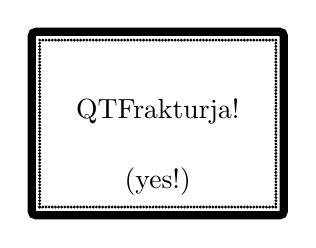
\begin{tikzpicture}
		\node at (0,0) {\fontsize{40}{40}\setmainfont{QTFraktur}ja!};
		\node at (0,-0.9) {(yes!)};
		
		\foreach \y in {-1.22, -1.18, ..., 0.9}
		{
			\fill (-1.5,\y) circle (0.2mm);
			\fill (1.5,\y) circle (0.2mm);
		}
		
		\foreach \x in {-1.5, -1.46, ..., 1.5}
		{
			\fill (\x,-1.22) circle (0.2mm);
			\fill (\x,0.9) circle (0.2mm);
		}
	
		\draw [line width=3, rounded corners = 1.5] (-1.6,-1.325) rectangle (1.6,1.005);
	\end{tikzpicture}
\end{document}